\documentclass{article}
\usepackage{listings}
\usepackage[utf8]{inputenc}
\usepackage{graphicx}
\renewcommand{\figurename}{Figura}
\usepackage{mathtools}
\usepackage{hyperref}
\usepackage[spanish]{babel}

\title{Informe de Estadística en Física Experimental: Guía 3 y 4}
\author{Andr\'es Babino}

\begin{document}
\maketitle
\section{Introducción}
El lenguaje utilizado para programar todas los ítems fue Python.
El código utilizado para generar los datos, gráficos y este mismo informe fue controlado con git, tiene licencia MIT y está almacenado en \url{https://github.com/ababino/efe}.

\section{Guía 3, Ejercicio 4, Ítem b}
En el gráfico de la figura \ref{fig:ej4b} se muestra la superposición de la distribución de Cauchy y la suma de dos Gaussianas.
Para x suficientemente chicos se ve que hay un acuerdo entre las dos distribucíones. 
Cuando $|x|$ es mayor a $6$ las colas gaussianas ya son menos pesadas que la de la disribución de Cauchy.


\begin{figure}
\centering
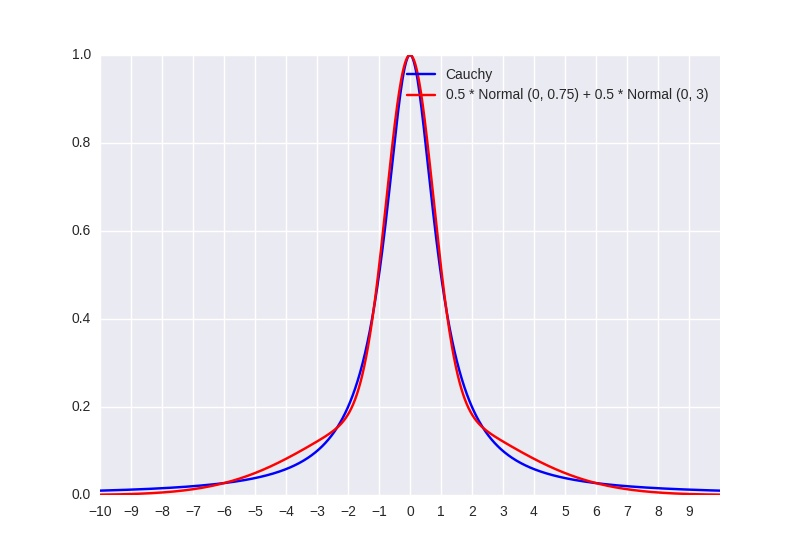
\includegraphics[width=0.75\textwidth]{ej4b.jpg}
\caption[]{Comparación entre la distribución de Cauchy y la suma de dos Gaussianas.}
\label{fig:ej4b}
\end{figure}

\section{Guía 3, Ejercicio 9, Ítem b}
Para generar una variable aleatoria con distribución exponencial busco una función de una variable aleatoria uniforme que tenga distribución exponencial:
$$f (x) = U(0, 1)$$
$$ g(y) = \lambda e^{-\lambda y}$$
$$g(y) \frac{dy}{dx} dx= f(x) dx $$

$$\lambda e^{-\lambda y} \frac{dy}{dx} = 1 $$

$$ y = -\frac{1}{\lambda} ln(1-x)$$

Entonces $y = -\frac{1}{\lambda} ln(1-x)$ es una variable aleatoria con distribución exponencial si $x$ tiene distribución uniforme.

En el gráfico de la figura \ref{fig:ej9b_1} se observa el resultado de implementar computacionalmente el método anterior.

En el gráfico de la figura \ref{fig:ej9b_2} se usaron bines de ancho $2$ para valores mayores a $15$.
En general para visualizar correctamente un histograma uno quiere que haya al menos un dato por bin. 
Si llamamos $n$ al número de resultdos que caen dentro de un determinado bin, $N$ al número total de datos y $f$ a la distribución de la variable aleatoria podemos estimar $n$ como:

$$ \hat n = N \int_{x_i}^{x_f} f(x) dx$$
$$ \hat n \sim N \Delta f(x_{intermedio}) $$

Donde aproximamos la función $f$ por una constante y llamamos $\Delta$ al ancho del bin.
Con este resultado podemos hallar una cota inferior al tamaño del bin pidiendo que $n>1$.

$$  \Delta > \frac{1}{N f(x_{intermedio})} $$

\begin{figure}
\centering
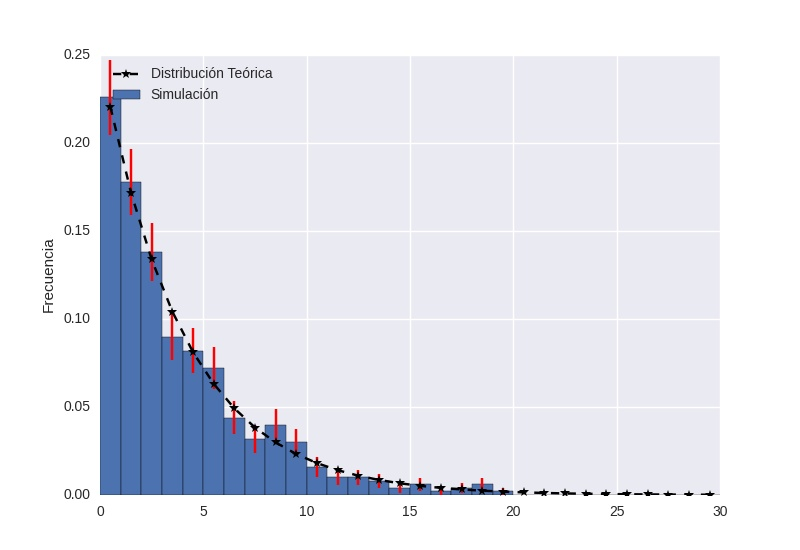
\includegraphics[width=0.75\textwidth]{ej9b_1.jpg}
\caption[]{}
\label{fig:ej9b_1}
\end{figure}

\begin{figure}
\centering
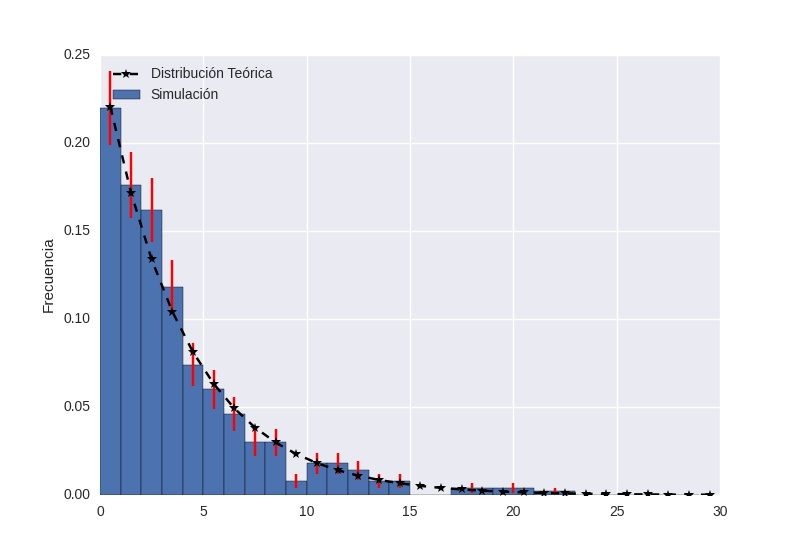
\includegraphics[width=0.75\textwidth]{ej9b_2.jpg}
\caption[]{}
\label{fig:ej9b_2}
\end{figure}

\section{Guía 4, Ejercicio 10}

\subsection{Ítem a}
Para calclular la densidad de probabilidad conjunta tengo que hallar la constante que normaliza a la densidad $\rho(r)$
$$f(r, \theta, \phi) = A \rho(r) $$
$$A = \frac{1}{\int_0^1 \int_0^{2\pi} \int_0^{\pi}\rho(r) sen(\theta) r^2 d\phi d\theta dr} $$
$$A = \frac{1}{\rho_0 \pi (4 - \pi)} $$
$$f(r, \theta, \phi) = \frac{1}{\pi (4 - \pi)} \frac{1}{1 + r^2} $$

\subsection{Ítem b}
Para calcular la distribución marginal de cada una de las coordenadas debo integrar la porbabilidad conjunta en todas las otras coordenadas. Siempre tengo que tener cuidado de usar el jacobiano adecuadamente.

$$f(r) = \int_0^{2\pi}\int_0^{\pi} f(r, \theta, \phi) sen(\theta) r^2 d\theta d\phi$$
$$f(r) = \frac{4 r^2}{(4 - \pi) (1 + r^2)}$$

$$f(\theta) = \int_0^1 \int_0^{2\pi}  f(r, \theta, \phi) sen(\theta) r^2 d\phi dr$$
$$f(\theta) = \frac{1}{2} sen(\theta)$$

$$f(\phi) = \int_0^1 \int_0^{\pi}  f(r, \theta, \phi) sen(\theta) r^2 d\theta dr$$
$$f(\theta) = \frac{1}{2\pi}$$

Las tres coordenadas son independientes pués se puede ver que la distribución conjunta es igual a la multiplicación de las marginales (si tenemos en cuenta el jacobiano).

\subsection{Ítem c}

Usando el método me Monte Carlo se simularon $1000$ vectores y a partir de ellos se calcularon sus coordenadas esféricas.
En los gráficos de las figuras \ref{g4ej10_r}, \ref{g4ej10_r} y \ref{g4ej10_r} se observa la comparación de esta simulación y las respectivas curvas teóricas. 


\begin{figure}
\centering
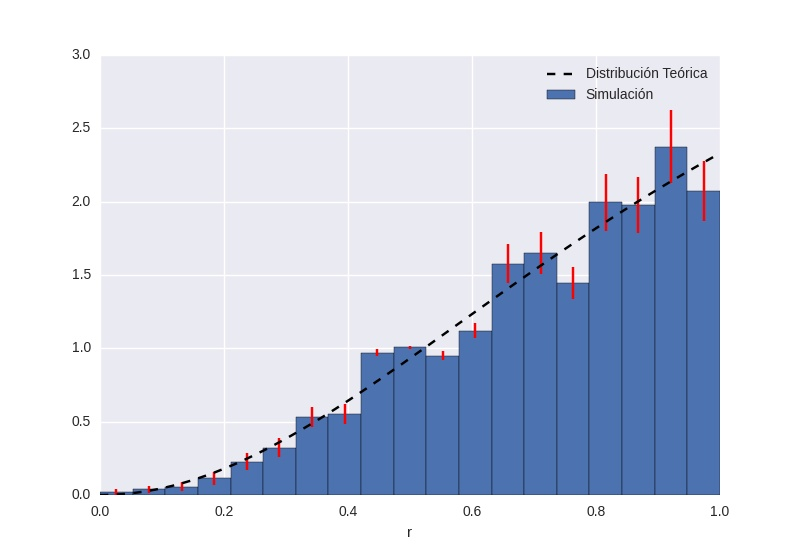
\includegraphics[width=0.75\textwidth]{g4ej10_r.jpg}
\caption[]{}
\label{fig:g4ej10_r}
\end{figure}

\begin{figure}
\centering
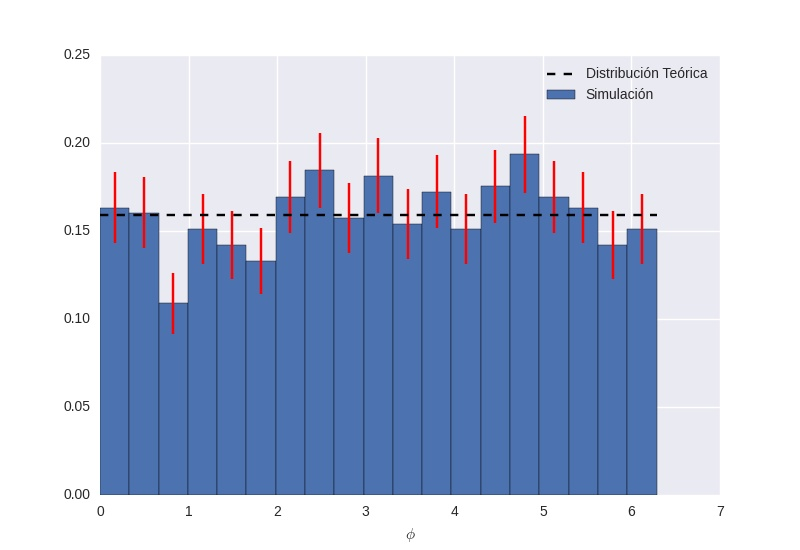
\includegraphics[width=0.75\textwidth]{g4ej10_phi.jpg}
\caption[]{}
\label{fig:g4ej10_r}
\end{figure}

\begin{figure}
\centering
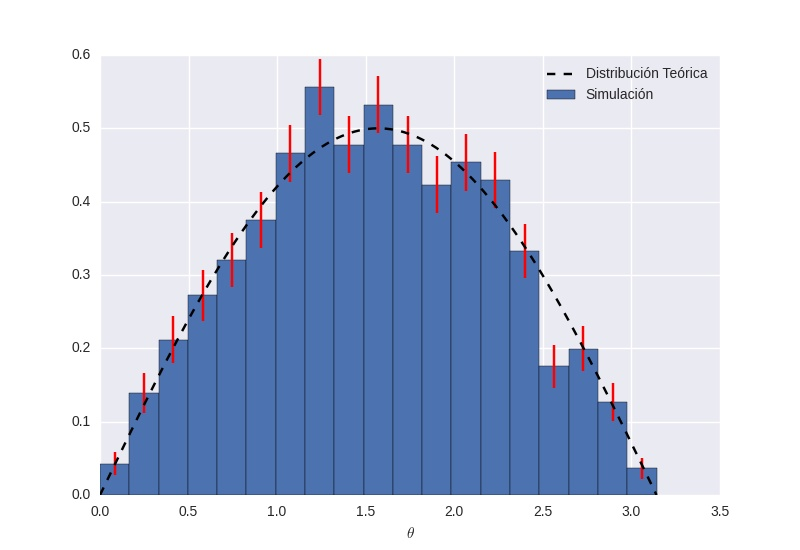
\includegraphics[width=0.75\textwidth]{g4ej10_theta.jpg}
\caption[]{}
\label{fig:g4ej10_r}
\end{figure}


\end{document}
